\section{Cloud-independent IoT over NDN}
\label{sec:ndn-iot}

\subsection{IoT and the cloud}
\label{sec:cloud-iot}

IoT applications and services often require a set of common services to be provided by the application-layer frameworks (shown in Fig.~\ref{fig:service-arch}):
\begin{itemize}
\item \emph{Identity management, authentication and authorization}, consisting of trust management for users, devices and services and, in connection-oriented models, access control;
\item \emph{Rendezvous and resource discovery}, enabling applications to find the devices and services they need;
\item \emph{Device management}, to handle onboarding, monitoring, configuration changes, software upgrades, etc. for constituent devices;
\item \emph{Application data messaging}, which supports data exchange through mechanisms including publish-subscribe (pub-sub), streaming, etc.;
\item \emph{Gateways to external network and services}, bridging IoT networks to other services such as data storage and analytics, as well as the public Internet mobile generally.
\end{itemize}

As we discussed in Section~\ref{sec:iot-ecosystems}, most IoT ecosystems today rely on the cloud to implement part or all of those framework services.
For example, in AWS IoT, the Amazon cloud service plays several critical roles that cover all of the above aspects of an IoT platform.
It acts as an identity provider, issuing security credentials for users and devices.  It provides authorization services, whereby device certificate issued by AWS contains the resource access policies prescribed by the user. It handles device management and rendezvous, where all devices in the IoT system register with and report to AWS, which also collects state for all devices and makes it available to applications.  All messages between IoT devices and services are tunneled through the cloud for pub-sub dispatching. AWS can host applications that consume the IoT data and trigger actions when certain events happen. Users can access the IoT network from public Internet, the messages are also tunneled through AWS via the message brokers.  

% The following is an application - 
%AWS IoT can store the device state persistently and analyze the IoT data using a variety of AWS services;

\begin{figure}[!t]
\centering
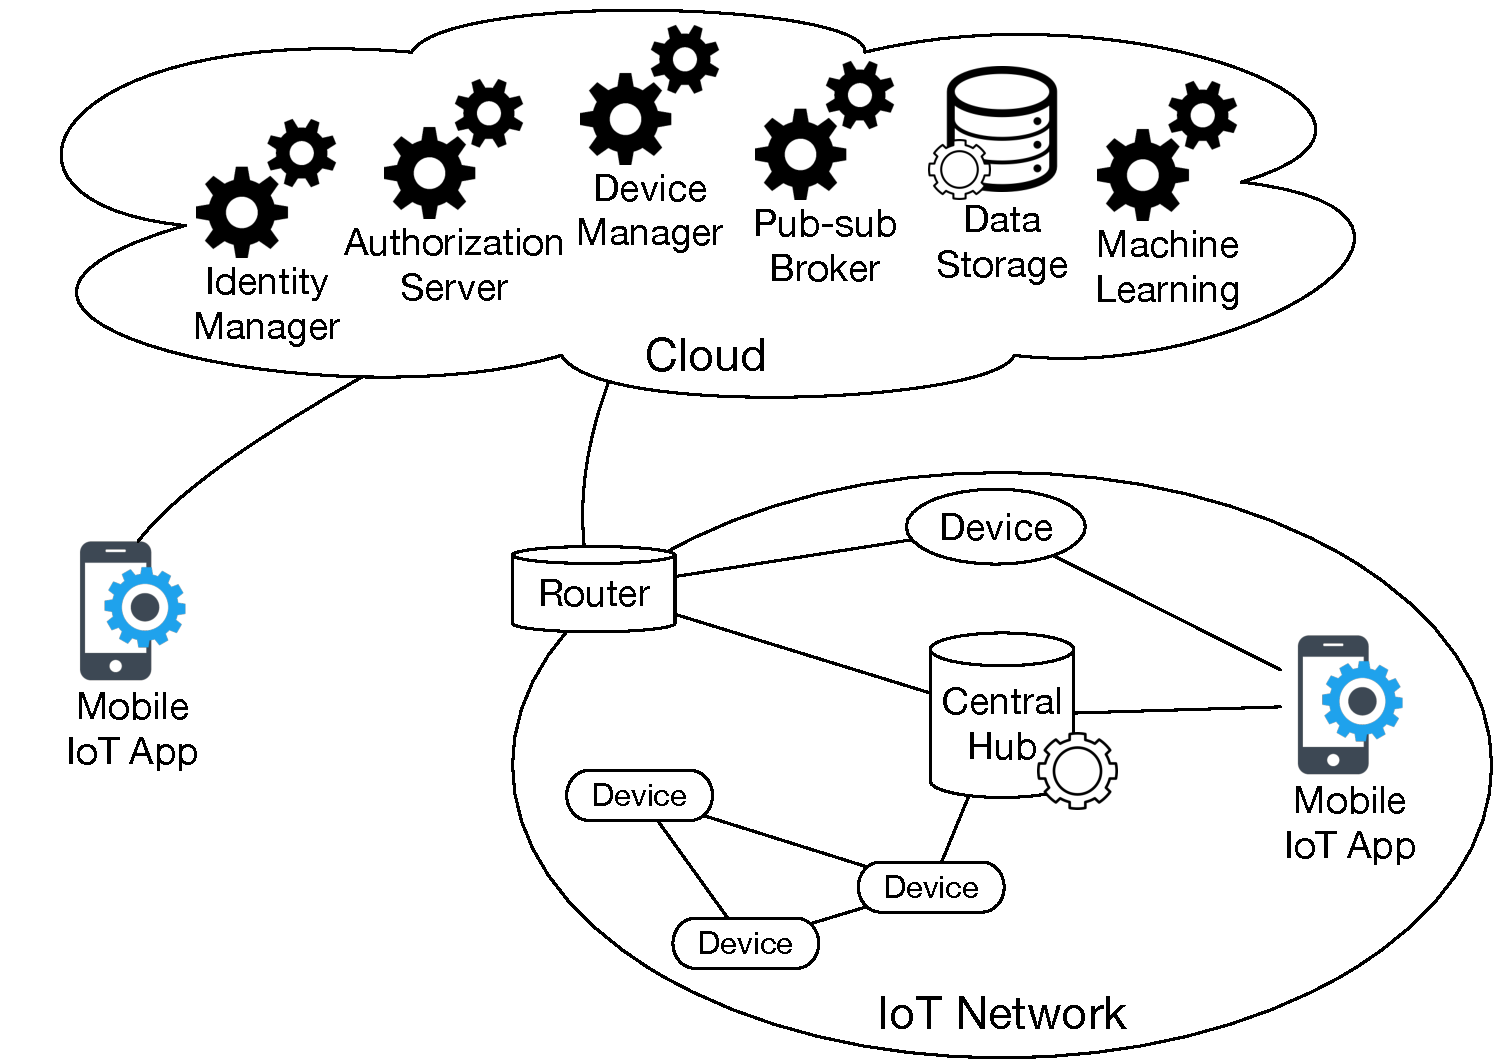
\includegraphics[width=0.9\columnwidth]{cloud-iot.pdf}
\caption{Typical cloud-centric IoT architecture}
\label{fig:cloud-iot}
\end{figure}

A typical cloud-centric IoT architecture is depicted in Fig.~\ref{fig:cloud-iot}.
%The cloud-centric model stems from the technical artifact that TCP/IP networking focuses on connecting different end nodes.
The cloud provides a convenient ``central hub'' for managing and interconnecting a large number of devices. 
While it simplifies the system configuration and management for the users by moving the control into the cloud, a cloud-centric IoT architecture sacrifices the opportunity of exploring proximal communications to achieve better reliability and efficiency.
The connectivity to the remote servers in the cloud becomes a single point of failure that unnecessarily affects the local services in the IoT network, and unnecessarily requires local data traverse the global network.
For example, for home IoT systems, a user cannot install or re-configure devices at home or access home network from public Internet if the connectivity from home to the cloud is down.
In ``human-in-the-loop'' application scenarios, control messages from the user's smartphone are first routed to the cloud for authentication and logging before being forwarded to the IoT device.
This extra latency is damaging for real-time, interactive applications, such as IoT-augmented home entertainment experiences. Further, the exposure of home devices to the global network unnecessarily is a security risk.
